\apendice{Documentación técnica de programación}

\section{Introducción}
Durante este anexo se describirá con detalle la documentación técnica de programación del proyecto. Esto incluye aspectos como la estructura de directorios que tiene, la instalación y uso del entorno de desarrollo, cómo llevar a cabo tanto su compilación, su instalación y ejecución, así como el método seguido para realizar las diferentes pruebas durante el desarrollo.
\section{Estructura de directorios}
Todos los materiales que forman el proyecto se encuentran en el repositorio de Github. Los directorios y archivos que contiene se organizan según la estructura que se describe a continuación:
\begin{itemize}
    \item \textbf{/docs}: Contiene los archivos relativos a la documentación del proyecto.
    \item \textbf{/TheOnlyOne}: es el directorio raíz de la estructura del juego.
        \begin{itemize}
        \item \textbf{/TheOnlyOne/Assets}: Contiene todos los archivos del propio desarrollo del juego, como scripts, modelos, animaciones, escenas, materiales y demás componentes que se importan o se crean en el proyecto para construir el videojuego.
            \begin{itemize}
            \item \textbf{/TheOnlyOne/Assets/Animations}:Contiene todos los archivos relacionados con las animaciones del juego. Esto incluye tanto los \textit{Animator controllers}, como los  \textit{Animation Clips}. Se clasifican en subcarpetas según el tipo de animaciones.
            \item \textbf{/TheOnlyOne/Assets/Editor Default Resources}: Contiene archivos necesarios para los scripts que requieran recursos cargados bajo demanda. Es utilizado por la base de datos.
            \item \textbf{/TheOnlyOne/Assets/ExternalDependencyManager}: Contiene algunas dependencias de paquetes que en este caso son usadas por Google para que Firebase funcione correctamente
            \item \textbf{/TheOnlyOne/Assets/Firebase}: Contiene los archivos de configuración principales de la base de datos de Firebase.
            \item \textbf{/TheOnlyOne/Assets/Global Volumes}: Contiene los diferentes perfiles de postprocesado del videojuego.
            \item \textbf{/TheOnlyOne/Assets/LeanTween}: Contiene los archivos relacionados con el paquete externo \textit{LeanTween}, importado para crear animaciones en algunos elementos de la interfaz.
            \item \textbf{/TheOnlyOne/Assets/Materials}: Contiene los diferentes materiales usados en el videojuego. Se dividen en subcarpetas según el elemento al que se le aplique el material.
            \item \textbf{/TheOnlyOne/Assets/Meshes}: Contiene las mallas de los modelos 3D utilizados, tanto propios como importados.
            \item \textbf{/TheOnlyOne/Assets/Parse}: Contiene archivos relativos al framework dotNet45 para la conexión con Firebase.
            \item \textbf{/TheOnlyOne/Assets/PhysicsMaterials}: Contiene diferentes materiales físicos utilizados en el videojuego.
            \item \textbf{/TheOnlyOne/Assets/Plugins}: Contiene ficheros necesarios para el funcionamiento de la base de datos en dispositivos con sistema operativo iOS.
            \item \textbf{/TheOnlyOne/Assets/Firebase}: Contiene los archivos de configuración principales de la base de datos de Firebase.
            \item \textbf{/TheOnlyOne/Assets/Prefabs}: Contiene todos los prefabs usados en el videojuego. Se dividen en subcarpetas según el ámbito del Prefab.
                \begin{itemize}
                \item \textbf{/TheOnlyOne/Assets/Prefabs/FinalPrefabs}: Almacena los prefabs que se instancian directamente en la escena.
                \end{itemize}
            \item \textbf{/TheOnlyOne/Assets/Presets}: Contiene archivos de configuración por defecto generados por unity para audio e imágenes.
            \item \textbf{/TheOnlyOne/Assets/QuickOutline}: Contiene los archivos relativos al paquete externo “QuickOutline” importado para crear un efecto de borde resaltado a los objetos.
            \item \textbf{/TheOnlyOne/Assets/Sci-Weapon Pack}: Contiene los modelos, texturas, materiales y demás ficheros del paquete externo importado relativo a las armas y packs del juego.
            \item \textbf{/TheOnlyOne/Assets/Scenes}: Contiene todas las escenas que componen el videojuego.
            \item \textbf{/TheOnlyOne/Assets/ScriptableObjects}: Contiene los diferentes scriptableObjects del juego, subdivididos por tipo
            \item \textbf{/TheOnlyOne/Assets/Scripts}: 
            \begin{itemize}
                \item \textbf{/TheOnlyOne/Assets/Scripts/	ScriptableObjectsGenerator}: Contiene las clases que definen los scriptableobjects del juego.
                \item \textbf{/TheOnlyOne/Assets/Scripts/NavMeshComponents}: Contiene los scripts y otros componentes para hacer que los enemigos puedan caminar por el terreno como se espera.
            \end{itemize}
            \item \textbf{/TheOnlyOne/Assets/Settings}: Contiene archivos de configuración gráfica y visual del proyecto.
            \item \textbf{/TheOnlyOne/Assets/ShaderGraphs}: Contiene los distintos shaders creados para crear los materiales especiales que hay en el videojuego.
            \item \textbf{/TheOnlyOne/Assets/Sounds}: Contiene todas las pistas de audio que se utilizan en la aplicación.
            \begin{itemize}
                \item \textbf{/TheOnlyOne/Assets/Sounds/Music}: Contiene la música que se reproduce de fondo en el videojuego
                \item \textbf{/TheOnlyOne/Assets/Sounds/SoundFX}: Contiene los diferentes efectos de sonido que se reproducen durante la ejecución del juego.
                \item \textbf{/TheOnlyOne/Assets/Sounds/UI}: Contiene los sonidos que se reproducen al interactuar con la interfaz, como los botones.
            \end{itemize}
            \item \textbf{/TheOnlyOne/Assets/Sprites&Textures}: Contiene todas las imágenes del videojuego divididas en subcarpetas según el elemento al que pertenecen. Incluye texturas, sprites, y cualquier archivo de imagen que se utilice.
            \item \textbf{/TheOnlyOne/Assets/StreamingAssets}: Contiene archivos especiales que no se deben modificar cuando se acceda a ellos. Se utiliza para almacenar el archivo que permite utilizar la base de datos en la versión de escritorio del proyecto.
            \item \textbf{/TheOnlyOne/Assets/TextMeshPro}: Contiene los archivos de configuración del paquete “TextMeshPro”, así como las fuentes y demás recursos utilizados.
        \end{itemize}
        \item \textbf{TheOnlyOne/Packages}: Contiene los archivos de configuración de los paquetes de Unity.
        \item \textbf{TheOnlyOne/ProjectSettings}: Contiene los archivos de configuración del proyecto necesarios para que el proyecto se pueda cargar en Unity.
        \item \textbf{TheOnlyOne/UserSettings}: Contiene archivos de configuración del usuario.
        \end{itemize}
\end{itemize}
\section{Manual del programador}
En este apartado se detallarán algunos pasos y aspectos relevantes que debe conocer el programador para poder desarrollar, compilar y ejecutar el proyecto.
\subsection{Instalación de Unity}
Para poder cargar el proyecto adecuadamente, lo primero que se debe hacer es instalar el motor de videojuegos Unity. Este será la base para realizar el resto de acciones asociadas al desarrollo.

Para ello, primero se debe acceder a la página oficial de Unity y descargar \textbf{\textit{Unity Hub}} (ver figura \ref{fig:DescargarUnity}), un centro de control para la gestión de los proyectos y de las diferentes versiones de Unity.

Hay que tener en cuenta los requisitos del sistema que pide el software para que se pueda ejecutar sin problemas.

\begin{figure}[h]
    \centering
    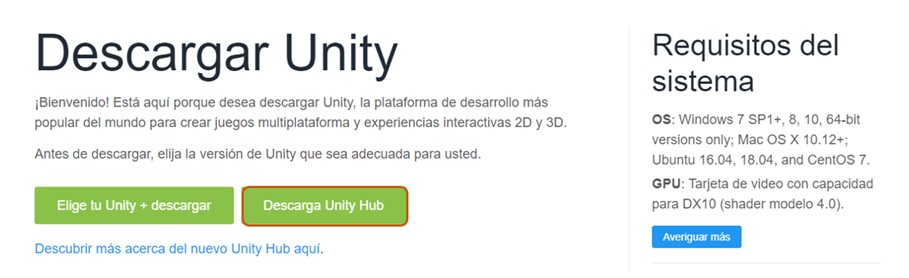
\includegraphics[scale=0.45]{img/UnityDownload.jpg}
    \caption{Página oficial de descargas de Unity}
    \label{fig:DescargarUnity}
    \end{figure}
    
Una vez en Unity Hub, se debe empezar por instalar el editor de Unity. Es importante que la versión de Unity que se descargue sea la misma que se utilizó al desarrollarse por el alumno para evitar errores o inconsistencias. En este caso, la versión utilizada es la \textit{2020.3.23f1}.

Es posible utilizar una versión diferente a la comentada, pero Unity es sensible y propenso a errores en algunos componentes cuando se utilizan versiones diferentes en un mismo proyecto.

Para instalarla, se debe acceder al apartado ``Installs'', y pulsar en ``Install Editor''. Después se elige la versión de Unity que se desea instalar (ver figura \ref{fig:InstalarUnity}).

\begin{figure}[h]
    \centering
    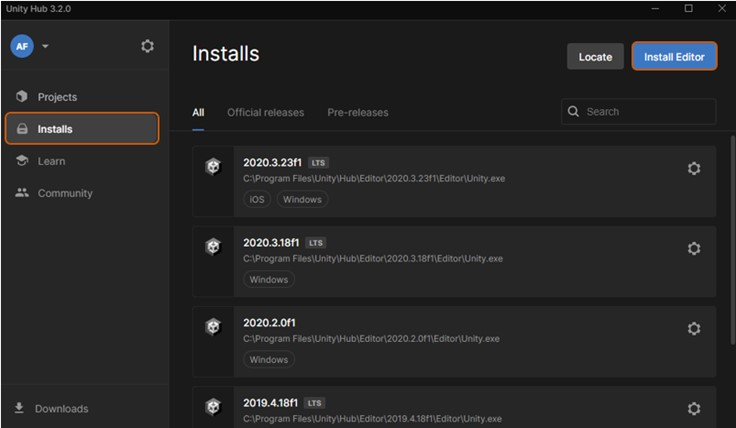
\includegraphics[scale=0.45]{img/UnityInstall.jpg}
    \caption{Instalar Unity desde Unity Hub}
    \label{fig:InstalarUnity}
    \end{figure}
    
Al instalar cualquier versión, se muestran los distintos módulos que se pueden añadir a la instalación de Unity (ver figura \ref{fig:MódulosUnity}). Para este proyecto, son necesarios los \textbf{módulos de compilación} de Windows y de Linux para que se pueda ejecutar en estas plataformas, como se requiere en los requisitos.\\
También es posible agregar estos módulos posteriormente, una vez Unity esté instalado en el sistema.

\begin{figure}[h]
    \centering
    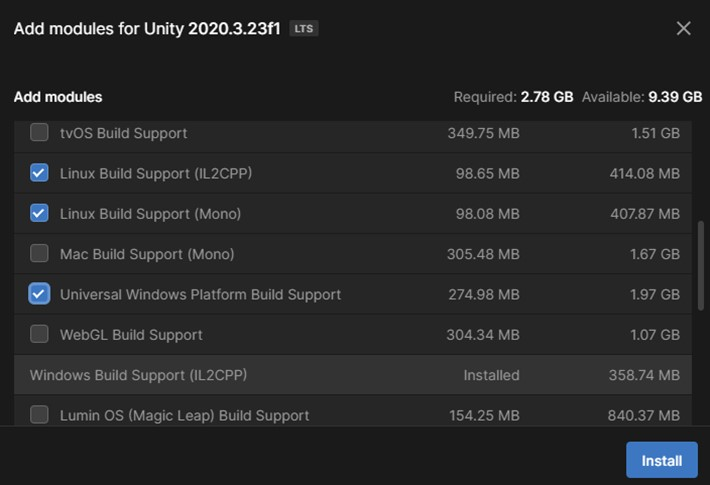
\includegraphics[scale=0.45]{img/UnityModules.jpg}
    \caption{Módulos de Unity}
    \label{fig:MódulosUnity}
    \end{figure}

\subsection{Importación del proyecto}
Unity hub permite añadir un proyecto nuevo o ya existente de varias formas. En este caso, lo que se debe hacer para importar el proyecto a Unity es descargarlo desde el repositorio de GitHub y guardarlo en algún directorio del ordenador.

Entonces en Unity Hub, en el apartado ``Projects'', se pulsa la opción de ``Open''. Se pedirá la ruta donde se encuentre el proyecto, y, una vez seleccionada, se añadirá el proyecto importado a la lista de proyectos disponibles (ver figura \ref{fig:ProyectosUnity}).

\begin{figure}[h]
    \centering
    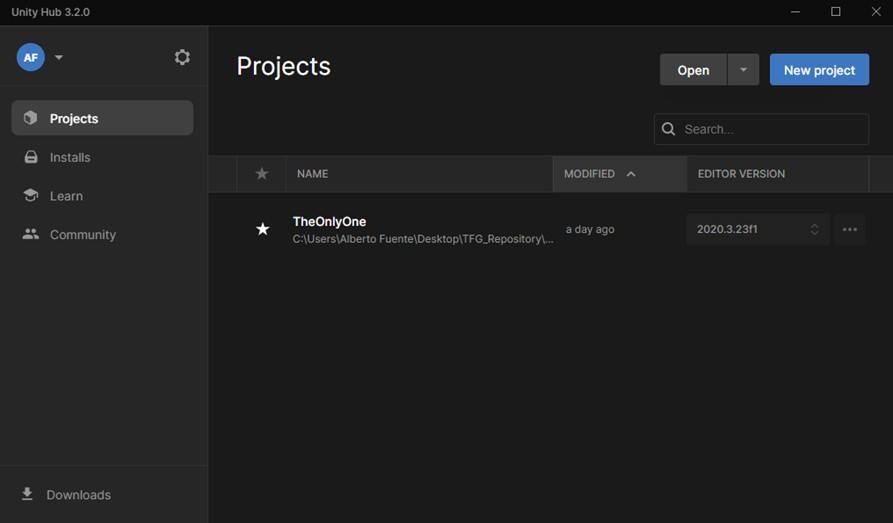
\includegraphics[scale=0.45]{img/UnityProjects.jpg}
    \caption{Ver proyectos disponibles de Unity}
    \label{fig:ProyectosUnity}
    \end{figure}
    
Junto al nombre del proyecto, se puede ver la fecha de la última vez que se modificó el proyecto, y la versión de Unity que utiliza. Esta se puede modificar si se desea ejecutar con otra más adecuada.

Para abrir el proyecto simplemente se pulsa en su nombre, y, tras unos segundos de carga, se podrá empezar a trabajar con él.

\subsection{Editor de Unity}
Una vez se acceda al proyecto, se cargará el editor de Unity. Este se compone de varios elementos y ventanas que son importantes de conocer para poder desarrollar el proyecto adecuadamente.

Cabe destacar que las posición y dimensiones de las ventanas no son fijas, y se pueden mover y redimensionar libremente a gusto del desarrollador. 

\begin{figure}[h]
    \centering
    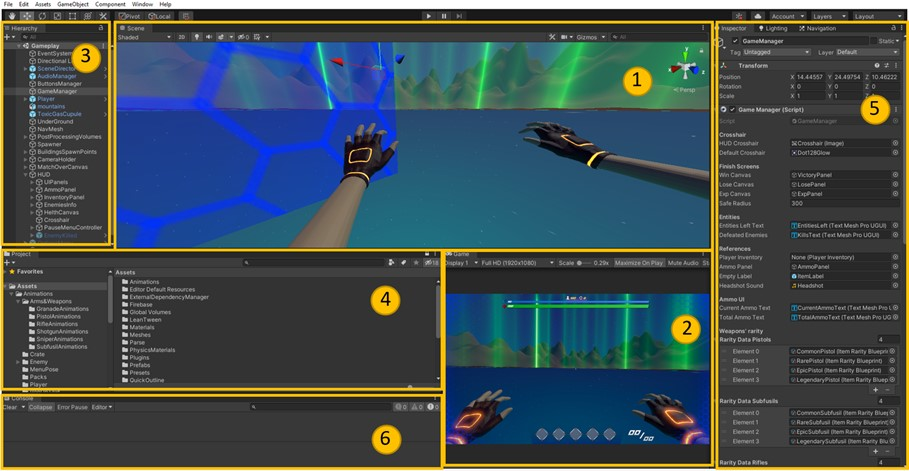
\includegraphics[scale=0.45]{img/UnityEditor.jpg}
    \caption{Editor de Unity}
    \label{fig:EditorUnity}
    \end{figure}
    
La figura \ref{fig:EditorUnity} sirve como leyenda para analizar cada una de las ventanas y elementos que más se utilizan en cualquier proyecto de Unity, descritos a continuación:
\begin{enumerate}
    \item \textbf{\textit{Scene}}. Esta ventana muestra un entorno 3D donde se pueden añadir los diferentes componentes disponibles para ir creando la escena. Dispone de una cámara virtual con la que se puede explorar este entorno libremente, alejándose o acercándose para examinar y editar cualquier elemento.\\
    Integra herramientas para modificar la posición, rotación y el tamaño de los gameobjects directamente desde la ventana.
    \item \textbf{\textit{Game}}. En la ventana de juego se muestra una vista previa de cómo se verá el juego una vez se ejecute. Resulta de gran valor para hacer pruebas de funcionamiento de las mecánicas o pruebas de disposición de los elementos de la interfaz.
    \item \textbf{\textit{Hierarchy}}. Es la jerarquía de objetos de la escena, es decir, esta ventana muestra todos los gameobjects y sus dependencias padre-hijo que existen dentro de la escena actual. Se puede utilizar para organizar y agrupar los gameobjects de la escena para gestionarlos más fácilmente.
    \item \textbf{\textit{Project}}. La ventana \textit{Project} contiene toda la jerarquía de assets y ficheros que se utilizan en el proyecto. Es una representación de la estructura de directorios y archivos que se almacena en disco relativa al proyecto, y contiene la información necesaria para poder cargarlo.
    
    Desde esta ventana se puede acceder a cualquier archivo del proyecto. Por ejemplo, se puede seleccionar cualquier escena dentro de la carpeta \textit{Assets/Scenes} para poder editarla. También se  puede utilizar para añadir elementos a la escena bien directamente como un gameobject o como componente de otros.\\
    Al arrastrar por ejemplo un Prefab desde esta ventana hasta la escena, se creará un nuevo gameobject en la Hierarchy, y ese gameobject ya formará parte de la escena.
    \item \textbf{\textit{Inspector}}. Esta ventana muestra toda la información y componentes de un objeto seleccionado, tanto de la \textit{Hierarchy} como de la carpeta Assets. Esta ventana permite ver las propiedades del objeto, añadir o eliminar componentes, activar o desactivarlos, o modificar sus valores.
    \item \textbf{\textit{Console}}. La consola de Unity funciona como cualquier consola de un entorno de desarrollo de software, mostrando todos los mensajes, las advertencias y los errores pertinentes que puedan surgir.\\
    Resulta de gran ayuda para depurar scripts, por ejemplo, ya que suele indicar la línea concreta en la que se encuentra el error, y cómo se ocasionó.
\end{enumerate}
De forma complementaria a las principales ventanas del editor, para poder editar y crear nuevos scripts, es recomendable disponer de un \textbf{IDE de programación} apropiado.

En el caso de Unity, lo habitual es utilizar \textit{Visual Studio}, ya que tiene varias funcionalidades para el desarrollo en Unity, como funciones de autocompletado o de depuración.\\
Para asociarlos, una vez en el proyecto, se debe seguir la ruta \textit{Edit>Preferences>External Tools}, y en la opción \textit{External Script Editor}, seleccionar el editor instalado en el ordenador que se desee utilizar (ver figura \ref{fig:HerramientasExternas}). En este caso, el editor y la versión elegidos ha sido Visual Studio Community 2022.

\begin{figure}[h]
    \centering
    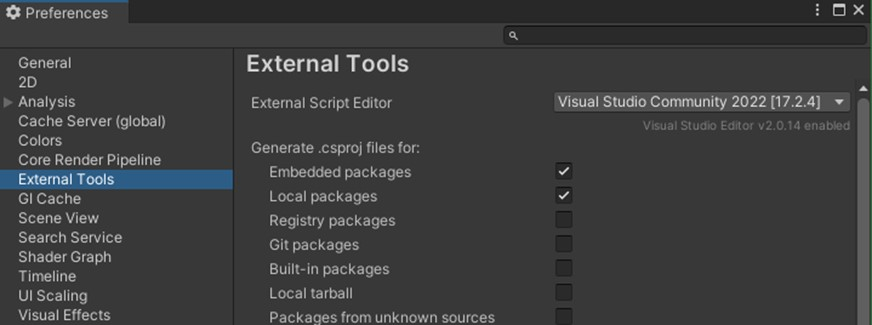
\includegraphics[scale=0.45]{img/ExternalTools.jpg}
    \caption{Asociar el proyecto a un IDE de programación}
    \label{fig:HerramientasExternas}
    \end{figure}
    
Una vez hecho esto, para editar un script basta con hacer doble clic sobre él, y automáticamente se abrirá Visual Studio para poder editarlo fácilmente. Al guardar los cambios realizados en el script, este se compilará de forma automática, y, si hay algún error o advertencia relacionados con el script, se mostrará en la consola del editor.

\section{Compilación, instalación y ejecución del proyecto}
Una vez se da por finalizado el desarrollo del videojuego, se debe compilar para poder exportarlo y ejecutarlo en otros dispositivos.
Para que la aplicación se compile en un producto final, simplemente hay que dirigirse al apartado \textit{Build Settings} dentro de la opción \textbf{File} del editor. 

Se abrirá una ventana de configuración (ver figura \ref{fig:OpcionesCompilacion}) donde se deben añadir todas las escenas que formen el juego. Es importante definir bien el orden en que se añaden estas escenas, ya que se les asignará un índice diferente a cada una en función del orden que sigan en esta ventana. 
\\
Esto será relevante a la hora de referenciar a las escenas en los scripts y porque la escena con el índice 0 será la primera en cargarse cuando se ejecute la aplicación.

\begin{figure}[h]
    \centering
    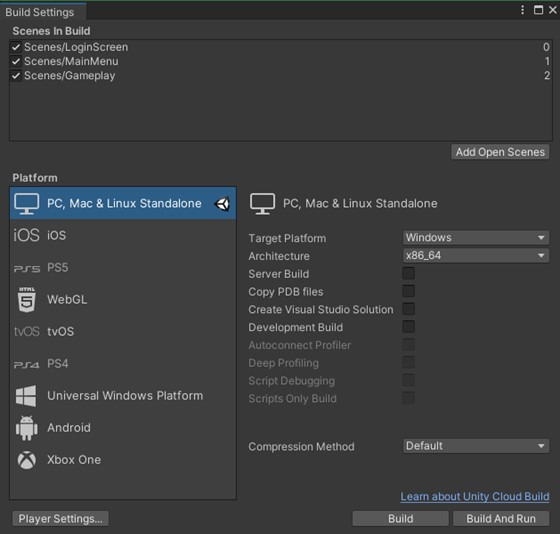
\includegraphics[scale=0.45]{img/BuildSettings.jpg}
    \caption{Opciones de compilación}
    \label{fig:OpcionesCompilacion}
    \end{figure}
    
Tras añadir las escenas en orden, se debe definir la plataforma para la que se desea compilar la aplicación, y, en su caso, el sistema operativo objetivo. Además, se pueden ajustar otras opciones como el tipo de arquitectura, o si se desea crear la solución para visual studio.
Una vez se seleccionen las opciones deseadas, simplemente se debe pulsar en ``Build'' para escoger el directorio donde se exportará el juego, almacenando todos los archivos necesarios para ejecutarlo (ver figura \ref{fig:FicherosJuego}).

\begin{figure}[h]
    \centering
    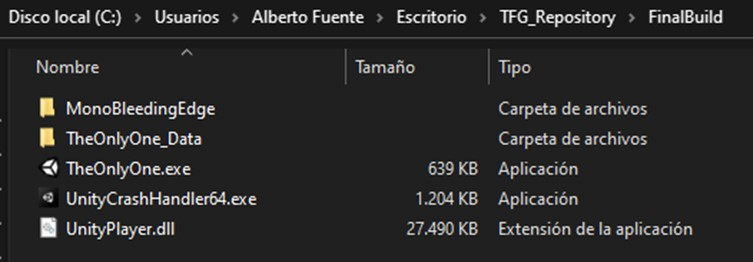
\includegraphics[scale=0.45]{img/GeneratedFiles.jpg}
    \caption{Ficheros generados en la compilación del juego}
    \label{fig:FicherosJuego}
    \end{figure}

\section{Pruebas del sistema}
Todo proyecto necesita hacer pruebas y testeos sobre sus diferentes componentes, así como del producto final, para comprobar que todo funciona como debe o si hay que hacer modificaciones en algunos elementos para tal fin.

La forma en la que se han puesto a prueba los elementos del videojuego es sencilla y ágil, permitiendo introducir cambios de forma conveniente en cada momento.
El editor de Unity permite ejecutar en cualquier momento la escena actual (siempre que no haya errores en los scripts), pulsando el botón \textbf{``Play''} de la parte superior del editor. 

Cuando se desea probar un elemento o parte de un elemento cuyo desarrollo se da por completado, se añade a la escena y se pulsa ``Play''. El usuario, a través de la ventana ``Game'', puede interactuar con el elemento como lo haría una vez se compilase el juego, para combropar que todo funciona como espera. Además, se puede complementar con el uso de la ventana ``Scene'', donde, incluso en tiempo de ejecución, el usuario puede navegar con la cámara virtual y seleccionar cada parte del elemento que se esté probando para ver en el Inspector si sus valores son los adecuados en cada momento.

Así, se testea de forma interactiva cada elemento que se quiera introducir de forma definitiva en la aplicación. Además, no hay que probar cada elemento uno por uno, sino que, si se quiere probar el comportamiento de varios elementos entre sí, simplemente se arrastran todos a la escena en la disposición deseada y al pulsar ``Play'', todo empezará a ejecutarse y a interactuar entre sí como lo haría en la versión definitiva.
Junto al botón de ``Play'' hay otro de \textbf{``Pause''} para poder parar momentáneamente la ejecución del programa y comprobar el estado de algún componente con detenimiento o introducir cambios en los valores de algunos elementos.

Cabe destacar que los cambios realizados durante la ejecución de las pruebas del programa, tanto si está en pausa como en modo ``Play'', se revierten al momento de parar completamente la ejecución, que se consigue volviendo a pulsar el botón de ``Play''. Por lo tanto, los cambios se tienen que hacer antes o después de ejecutar la aplicación.

Además, junto al botón de pausa hay un botón que se podría llamar \textbf{``Next frame''}, y que sirve para avanzar la ejecución del programa frame a frame cada vez que se pulse. Con esta funcionalidad se pueden testear elementos con un comportamiento más complejo o veloz que requieran más detenimiento para analizarlos.
 
\begin{figure}[h]
    \centering
    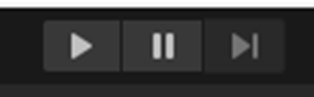
\includegraphics[scale=0.45]{img/PlayPauseNextframe.jpg}
    \caption{Botones de ``play'', ``pause'' y ``next frame''}
    \label{fig:}
    \end{figure}

Esta forma de realizar pruebas responde muy bien a la metodología Kanban, seguida en este proyecto, ya que permite hacer constantes pruebas durante el desarrollo sin tener que esperar a una fase específica de pruebas.
